Die Photodiode hat von dem Spalt den Abstand
\begin{align*}
  L=\SI{0,9}{m}.
\end{align*}
Der Laser leuchtet mit einer Wellenlänge von
\begin{align*}
  \lambda=\SI{635e-9}{nm}.
\end{align*}
Die Messung des Dunkelstroms ergibt:
\begin{align*}
  I_{\text{du}}=\SI{0,58}{nA}.
\end{align*}
Bei allen nachfolgenden Intensitäten wird der Dunkelstrom $I_{du}$ abgezogen um den realen Wert zu erhalten.
Die maximale Intensität jeder Messung wird als Nullpunkt genommen.
\subsection{Einzelspalt 1}
Die Spaltbreite ist gegeben als:
\begin{align*}
  b=\SI{0,022e-3}{m}.
\end{align*}
Die gemessenen Werte sind in der Tabelle \ref{tab:1a} und in der Abbildung \ref{fig:1a} dargestellt.\\
Mit Phython wird eine Ausgleichsrechnung nach der Form der Gleichung \ref{eqn:einzelspalt} bestimmt.
Die durch Python errechnete Spaltbreite beträgt:
\begin{align*}
  b=\SI{0,045\pm0,001e-3}{m}.
\end{align*}
\begin{table}[h!]
  \centering
  \caption{Messwerte für den Einzelspallt mit $b=\SI{0,022e-3}{m}$}
  \label{tab:1a}
  \begin{tabular}{c c c c}
    \toprule
       Auslenkung /mm  & Intensität /nA & Auslenkung /mm& Intensität /nA  \\
    \midrule

	  0,00	  	& 7,92 & -23,94	  	& 0,52\\
	 -0,14	  	& 7,92 & -24,44	    &	0,52\\
	 -1,44	  	& 7,72 & -24,94	    &	0,50\\
	 -1,94	  	& 7,42 & -25,44	    &	0,50\\
	 -2,44	  	& 7,02 & -25,94	  	& 0,43\\
	 -2,94	  	& 6,62 & -26,44	  	& 0,42\\
	 -3,44	  	& 6,12 & -26,94	  	& 0,42\\
	 -3,94	  	& 5,62 & 0,06	    	& 8,62\\
	 -4,44	  	& 5,02 & 0,56	    	& 8,42\\
	 -4,94	  	& 4,42 & 1,06	    	& 8,12\\
	 -5,44	  	& 3,82 & 1,56	    	& 7,82\\
	 -5,94	  	& 3,32 & 2,06	    	& 7,22\\
	 -6,44	  	& 2,82 & 3,06	    	& 6,22\\
	 -6,94	  	& 2,32 & 4,06	    	& 6,22\\
	 -7,44	  	& 1,92 & 5,06	    	& 5,12\\
	 -7,94	  	& 1,62 & 6,06	    	& 4,02\\
	 -8,44	  	& 1,32 & 7,06	    	& 2,22\\
	 -8,94	  	& 1,12 & 8,06	    	& 1,62\\
	 -9,44	  	& 0,92 & 8,56	    	& 1,27\\
	 -9,94	  	& 0,80 & 9,06	    	& 1,12\\
	 -10,44	  	& 0,72 & 9,56	    	& 0,97\\
	 -10,94	  	& 0,72 & 10,06    	& 0,87\\
	 -11,44	  	& 0,72 & 10,56	  	& 0,82\\
	 -11,94	  	& 0,72 & 11,06	  	& 0,77\\
	 -12,44	  	& 0,75 & 11,56	  	& 0,72\\
	 -12,94	  	& 0,75 & 12,06	  	& 0,72\\
	 -13,44	  	& 0,77 & 12,56	  	& 0,68\\
	 -13,94	  	& 0,77 & 13,06	  	& 0,68\\
	 -14,44	  	& 0,77 & 13,56	  	& 0,67\\
	 -14,94	  	& 0,77 & 14,06	  	& 0,67\\
	 -15,44	  	& 0,72 & 14,56	  	& 0,62\\
	 -15,94	  	& 0,67 & 15,06	  	& 0,62\\
	 -16,44	  	& 0,62 & 15,56	  	& 0,57\\
	 -16,94	  	& 0,57 & 16,06	  	& 0,52\\
	 -17,44	  	& 0,52 & 16,56	  	& 0,47\\
	 -17,94	  	& 0,47 & 17,06	  	& 0,42\\
	 -18,44	  	& 0,42 & 17,56	  	& 0,37\\
	 -18,94	  	& 0,42 & 18,06	  	& 0,32\\
	 -19,44	  	& 0,37 & 18,56	  	& 0,27\\
	 -19,94	  	& 0,37 & 19,06	  	& 0,27\\
	 -20,44	  	& 0,42 & 19,56	  	& 0,22\\
	 -20,94	  	& 0,42 & 20,56	  	& 0,17\\
	 -21,44	  	& 0,42 & 21,56	  	& 0,17\\
	 -21,94	  	& 0,42 & 22,56	  	& 0,17\\
	 -22,44	  	& 0,47 & 23,56	  	& 0,17\\
	 -22,94	    &	0,47 & 24,56	  	& 0,17\\
	 -23,44	  	& 0,50 & 25,56	  	& 0,17\\



\bottomrule
\end{tabular}
\end{table}

\begin{figure}
  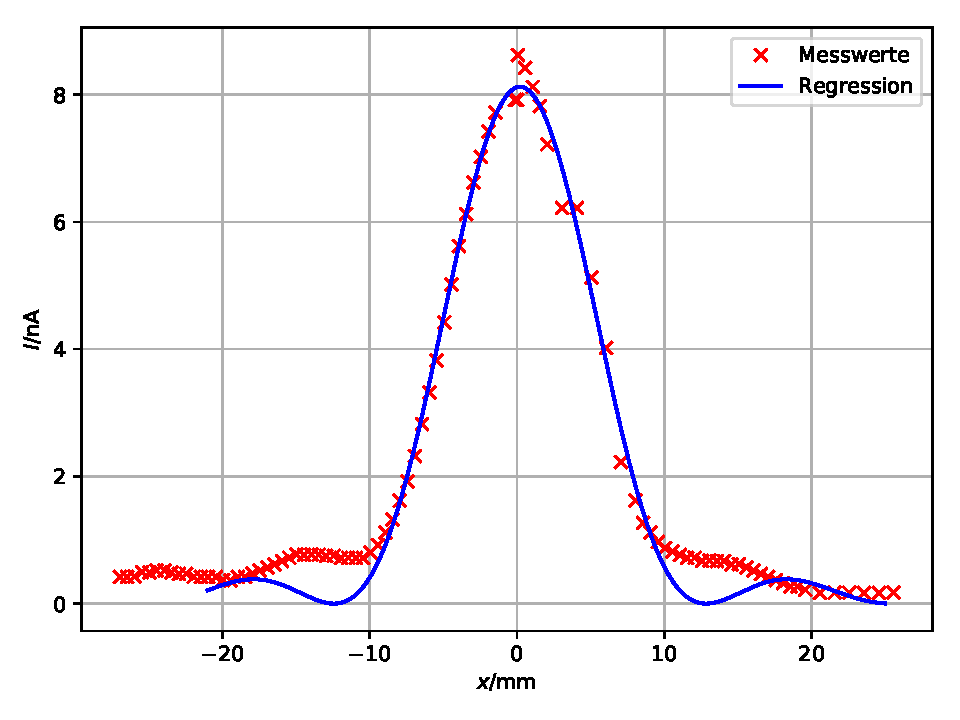
\includegraphics{1a.pdf}
  \caption{Einzelspalt 1}
  \label{fig:1a}
\end{figure}
\FloatBarrier
\subsection{Einzelspalt 2}
Die Spaltgröße ist gegeben als:
\begin{align*}
  b=\SI{0,1e-3}{m}
\end{align*}
Die gemessenen Werte sind in der Tabelle \ref{tab:1b} und in der Abbildung \ref{fig:1b} dargestellt.\\
Mit Phython wird erneut eine Ausgleichsrechnung mit Gleichung \ref{eqn:einzelspalt} ausgeführt.
Die von Python berechnete Spaltbreite beträgt:
\begin{align*}
  b = \SI{0.29\pm0.01e-3}{m}.
\end{align*}
\begin{table}[h!]
  \centering
  \caption{Messwerte für den Einzelspallt mit $b=\SI{0,1e-3}{m}$}
  \label{tab:1b}
  \begin{tabular}{c c c c}
    \toprule
       Auslenkung /mm  & Intensität /nA & Auslenkung /mm  & Intensität /nA  \\
    \midrule

    0,00		&299,42&-&-\\
   -0,50		&339,42&0,50		&179,42\\
   -1,00		&234,42&1,00		&74,42\\
   -1,50		&99,42&1,50		&44,42\\
   -2,00		&43,42&2,00		&29,42\\
   -1,31		&40,42&2,50		&24,42\\
   -2,50		&42,42&3,00		&21,92\\
   -3,00		&42,42&3,50		&19,42\\
   -3,50		&37,42&4,00		&16,92\\
   -4,00		&29,42&4,20		&16,92\\
   -4,50		&19,42&4,50		&18,42\\
   -5,00		&13,42&4,79		&18,92\\
   -5,19		&13,42&5,00		&17,92\\
   -5,50		&15,42&5,50		&14,42\\
   -6,00		&19,42&6,00		&12,92\\
   -6,50		&25,42&6,50		&13,42\\
   -7,00		&29,92&7,00		&14,92\\
   -7,13		&31,42&7,50		&15,42\\
   -7,50		&26,92&8,00		&14,92\\
   -8,00		&14,92&8,50		&10,92\\
   -8,50		&12,92&9,00		&8,42\\
   -9,00		&11,92&9,50		&6,42\\
   -9,50		&17,92&10,00		&5,82\\
   -9,73		&18,42&10,50		&4,62\\
   -10,0		&17,42&11,00		&3,92\\
   -10,5		&13,42&11,50		&3,62\\



   \bottomrule
\end{tabular}
\end{table}

\begin{figure}
  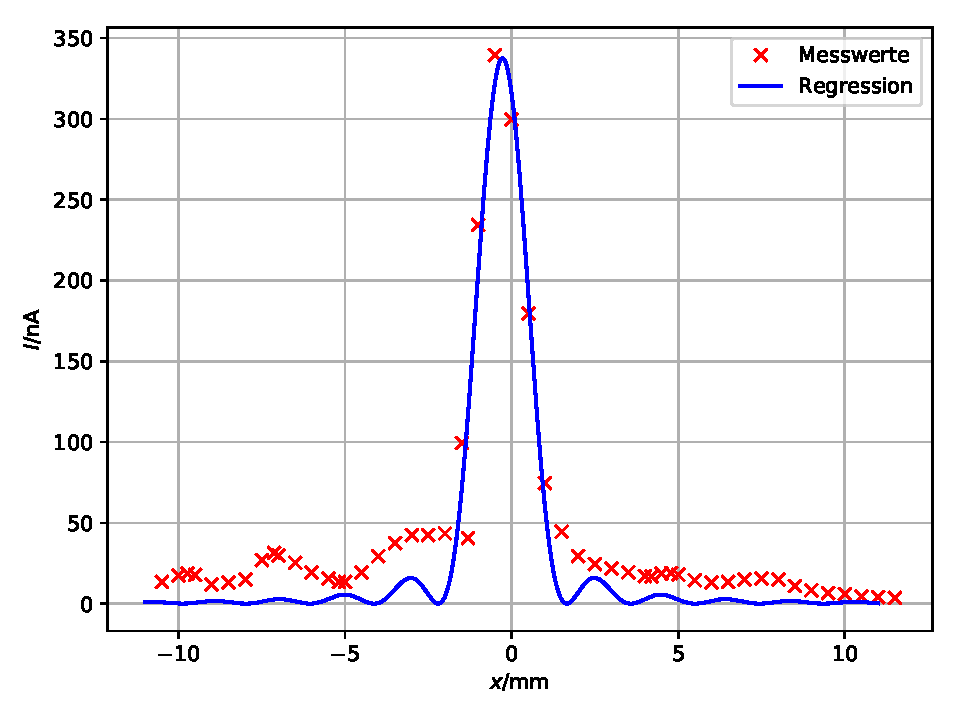
\includegraphics{1b.pdf}
  \caption{Einzelpalt 2}
  \label{fig:1b}
\end{figure}
\FloatBarrier

\subsection{Doppelspalt}
Die Spaltgrößen $b$ und der Spaltabstand $s$ sind gegeben als:
\begin{align*}
  b=\SI{0,15e-3}{m}\\
  g=\SI{0,25e-3}{m}.
\end{align*}
Die gemessenen Werte sind in der Tabelle \ref{tab:2} und in der Abbildung \ref{fig:2} dargestellt.
Die nicht-lineare Ausgleichsrechnung nach Gleichung \ref{eqn:doppelspalt} wird mit Python bestimmt.
\begin{table}[h!]
  \centering
  \caption{Messwerte für den Doppelspalt mit $b=\SI{0,15e-3}{m}$ und $g=\SI{0,25e-3}{m}$}
  \label{tab:2}
  \begin{tabular}{c c c c}
    \toprule
       Auslenkung /mm  & Intensität /nA & Auslenkung /mm  & Intensität /nA  \\
    \midrule



    0,00		& 189,42&0,00		& 179,42\\
   -0,25		& 194,42&0,25		& 134,42\\
   -0,50		& 174,92&0,50		& 79,42\\
   -0,75		& 129,92&0,75		& 45,42\\
   -1,00		& 85,42& 1,00		& 34,42\\
   -1,25		& 57,42& 1,25		& 38,42\\
   -1,50		& 52,42& 1,50		& 47,42\\
   -1,75		& 59,42& 1,73		& 51,42\\
   -2,00		& 66,42& 1,75		& 51,42\\
   -2,25		& 66,42& 2,00		& 51,42\\
   -2,50		& 61,42& 2,25		& 47,42\\
   -2,75		& 57,42& 2,50		& 47,42\\
   -3,00		& 57,42& 2,75		& 49,42\\
   -3,25		& 57,42& 3,00		& 46,42\\
   -3,50		& 52,42& 3,25		& 42,42\\
   -3,75		& 42,42& 3,50		& 30,42\\
   -4,00		& 31,42& 3,75		& 22,92\\
   -4,25		& 23,42& 4,00		& 17,92\\
   -4,50		& 21,42& 4,25		& 14,32\\
   -4,75		& 26,42& 4,35		& 13,92\\
   -5,00		& 31,42& 4,50		& 13,92\\
   -5,25		& 33,42& 4,75		& 14,42\\
   -5,50		& 30,42& 5,00		& 14,32\\
   -5,75		& 24,42& 5,25		& 13,42\\
   -6,00		& 18,42& 5,50		& 11,92\\
   -6,25		& 12,42& 5,75		& 10,92\\
   -6,50		& 9,42& 5,76		& 10,92\\
   -6,72		& 9,22& 6,00		& 11,42\\
   -6,75		& 9,32& 6,25		& 12,92\\
   -7,00		& 11,42& 6,50		& 14,42\\
   -7,25		& 14,92& 6,75		& 16,42\\
   -7,50		& 17,92& 7,00		& 16,92\\
   -7,73		& 18,42& 7,25		& 16,22\\
   -7,73		& 18,92& 7,50		& 13,92\\
   -8,00		& 17,42& 7,75		& 13,92\\
   -8,25		& 15,42& 8,00		& 9,22\\
   -8,50		& 12,92& 8,15		& 8,62\\
   -8,75		& 11,92& 8,25		& 8,42\\
   -9,00		& 11,97& 8,50		& 9,02\\
   -9,25		& 12,92& 8,75		& 9,92\\
   -9,50		& 14,42& 9,00		& 10,92\\
   -9,75		& 9,92& 9,25		& 10,42\\
   -10,00		& 9,92& 9,50		& 8,82\\
   -        &   - & 9,75		& 7,22\\
   -        &   - & 10,00	& 6,42\\



   \bottomrule
\end{tabular}
\end{table}

\begin{figure}
  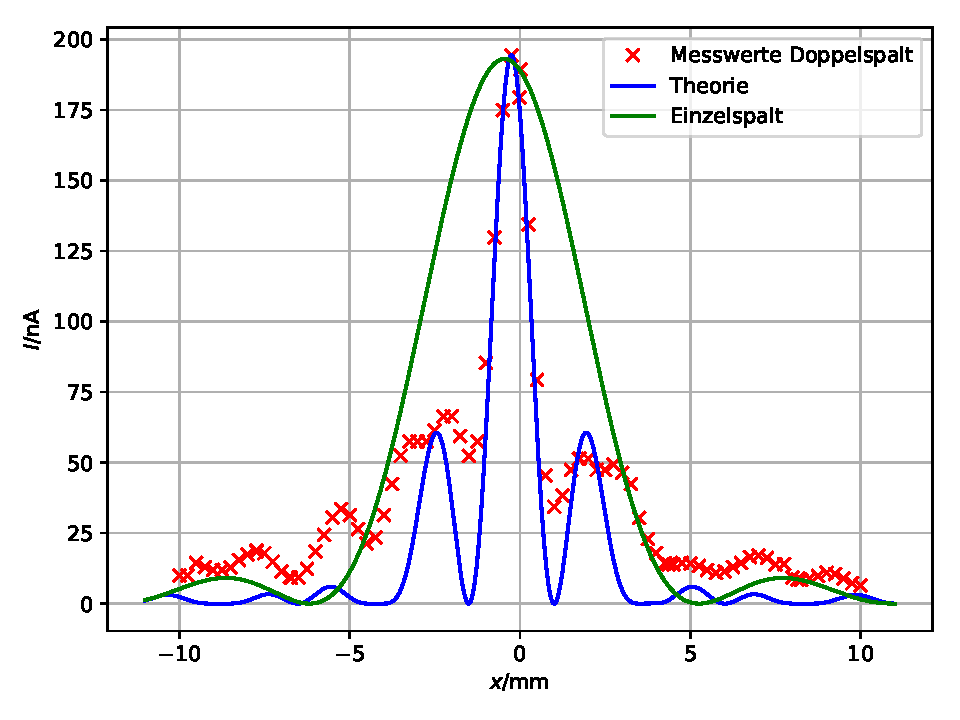
\includegraphics{2.pdf}
  \caption{Doppelspalt}
  \label{fig:2}
\end{figure}
\FloatBarrier
